\section{Lmapper}
\subsection{Intro}
The architecture has been inspired to the previous implementation of Daniel M\"ullner \cite{pythonmapper}. Compared to Kepler Mapper, this architecture is complex but more modular. However, the API of such package is too complex to use, and thus we aimed to design a simpler API similar to Kepler Mapper's one.\\
The approach followed for the development of this package was a test-driven approach: first a basic test for the package was written, and then the code necessary to make it work was developed. Once the first test was passed, this procedure was iterated with a more complex test containing more advanced features. This approach was chosen since in this way the development was always guided by a specific goal (pass the test).
We present here under the first two tests that were designed and we comment them.

\paragraph{test 1}
\begin{lstlisting}[language=Python, caption=First test for Mapper]
import lmapper as lm
from lmapper.filter import Projection
from lmapper.cover import UniformCover
from lmapper.cluster import Linkage
from lmapper.cutoff import FirstGap
from lmapper.datasets import circles

def main():
	filter = Projection(ax=0)
	cover = UniformCover(nintervals=15,
										     overlap=0.4)
	cutoff = FirstGap(0.05)
	cluster = Linkage(method='single',
									 metric="euclidean",
									 cutoff=cutoff)
	mapper = lm.Mapper(data=circles,
											filter=filter,
	 										cover=cover,
											cluster=cluster)
	mapper.fit()
	mapper.plot()


if __name__ == "__main__":
main()

\end{lstlisting}
This test shows the main components and design choices of the package. 
\paragraph{Import statements}
The code would be structured in a pure OOP fashion. The package would have been composed by five modules: \_mapper.py, filter.py, cover.py, cluster.py, cutoff.py.  Each module contains the definitions of the classes implementing the corresponding algorithms. 
\paragraph{main()}
First, one object for the filter, one object for the cover, one object for the cutoff method used in the clustering step, one object for the clustering step are instantiated. Given the many parameters of Mapper, in this way each step of the Mapper pipeline is isolated in an object that contains its set of parameters, avoiding long lists of parameters that could make the API confused.\\
These objects (filter, cover, cluster) are then used to instantiate a mapper object together with the data that has to be analyzed. The mapper object has to expose to the client user two methods: fit() and plot().\\
It can be seen that such test looks more readable that the code necessary for PyMapper, but however it let the user set all the parameters that Kepler Mapper hides and does not let the user choose. Plus, the package is clearly modular: if in the future more algorithms would be necessary (i.e. a new way of building a cover, or a new clustering algorithm) it would be necessary to implement a corresponding new class respecting the API of the backend to correctly interact with the other modules, expose it to the user and all the future patches of the package would make all the old client code still compatible.\\

\paragraph{test 2}
\begin{lstlisting}[language=Python, caption=Second test for Mapper]
import lmapper as lm
from lmapper.filter import Projection
from lmapper.cover import UniformCover
from lmapper.cluster import Linkage
from lmapper.cutoff import FirstGap
from lmapper.datasets import circles

def main():
	filter = Projection(ax=0)
	cover = UniformCover(nintervals=15,
											 overlap=0.4)
	cutoff = FirstGap(0.05)
 	cluster = Linkage(method='single',
									 metric="euclidean",
									 cutoff=cutoff)
	mapper = mp.Mapper(data=circles,
											 filter=filter,
											 cover=cover,
											 cluster=cluster)
	mapper.fit()
	mapper.plot()
	
	cluster = Linkage(method='average',
									 metric='correlation',
									 cutoff=cutoff)
	mapper.set_params(cluster=cluster)
	mapper.fit()
	mapper.plot


if __name__ == "__main__":
main()

\end{lstlisting}
This test was designed to solve the following issue: Mapper has a lot of parameters, and to set them correctly a lot of trial-and-error has to be done by the user to find a good choice of parameters. All the previous implementations taken in exam in this work, when a parameter is changed, need to recalculate everything from scratch, making the trial-and-error procedure really slow and annoying. However, Mapper is an algorithm that has a clear pipeline
\begin{enumerate}
	\item Calculate the filter values
	\item Calculate the pull-back cover
	\item Cluster each element of the pullback cover
	\item Build the simplicial complex from the elements of the pullback cover
\end{enumerate}
Each one of these steps is completely independent from the previous ones; this means that if we fit a Mapper object, and then we decide to try to fit it with a change of the clustering method, there's no need to recompute the filter values and the pullback cover, and the computations could restart from step (3). To enable this we need to design the Mapper class to store all the intermediate information needed to restart the computation from whichever step, and make it "aware" of the changes to the previous set of parameters through the method set\_params().\\
We want to underline that this design represents a completely new feature that was never implemented before in our knowledge.\\
\paragraph{Base architecture}
In figure \ref{fig:basearchitecture} the architecture for a first implementation of the package necessary to pass the first two tests is illustrated. The final version of the package is more complex, but this is sufficient to illustrate the high level design choices that were respected during the whole development. The real architecture will be discussed in details later on.\\
\begin{figure}[h]
	\caption{Simplified Mapper Architecture (simplified)}
	\centering
	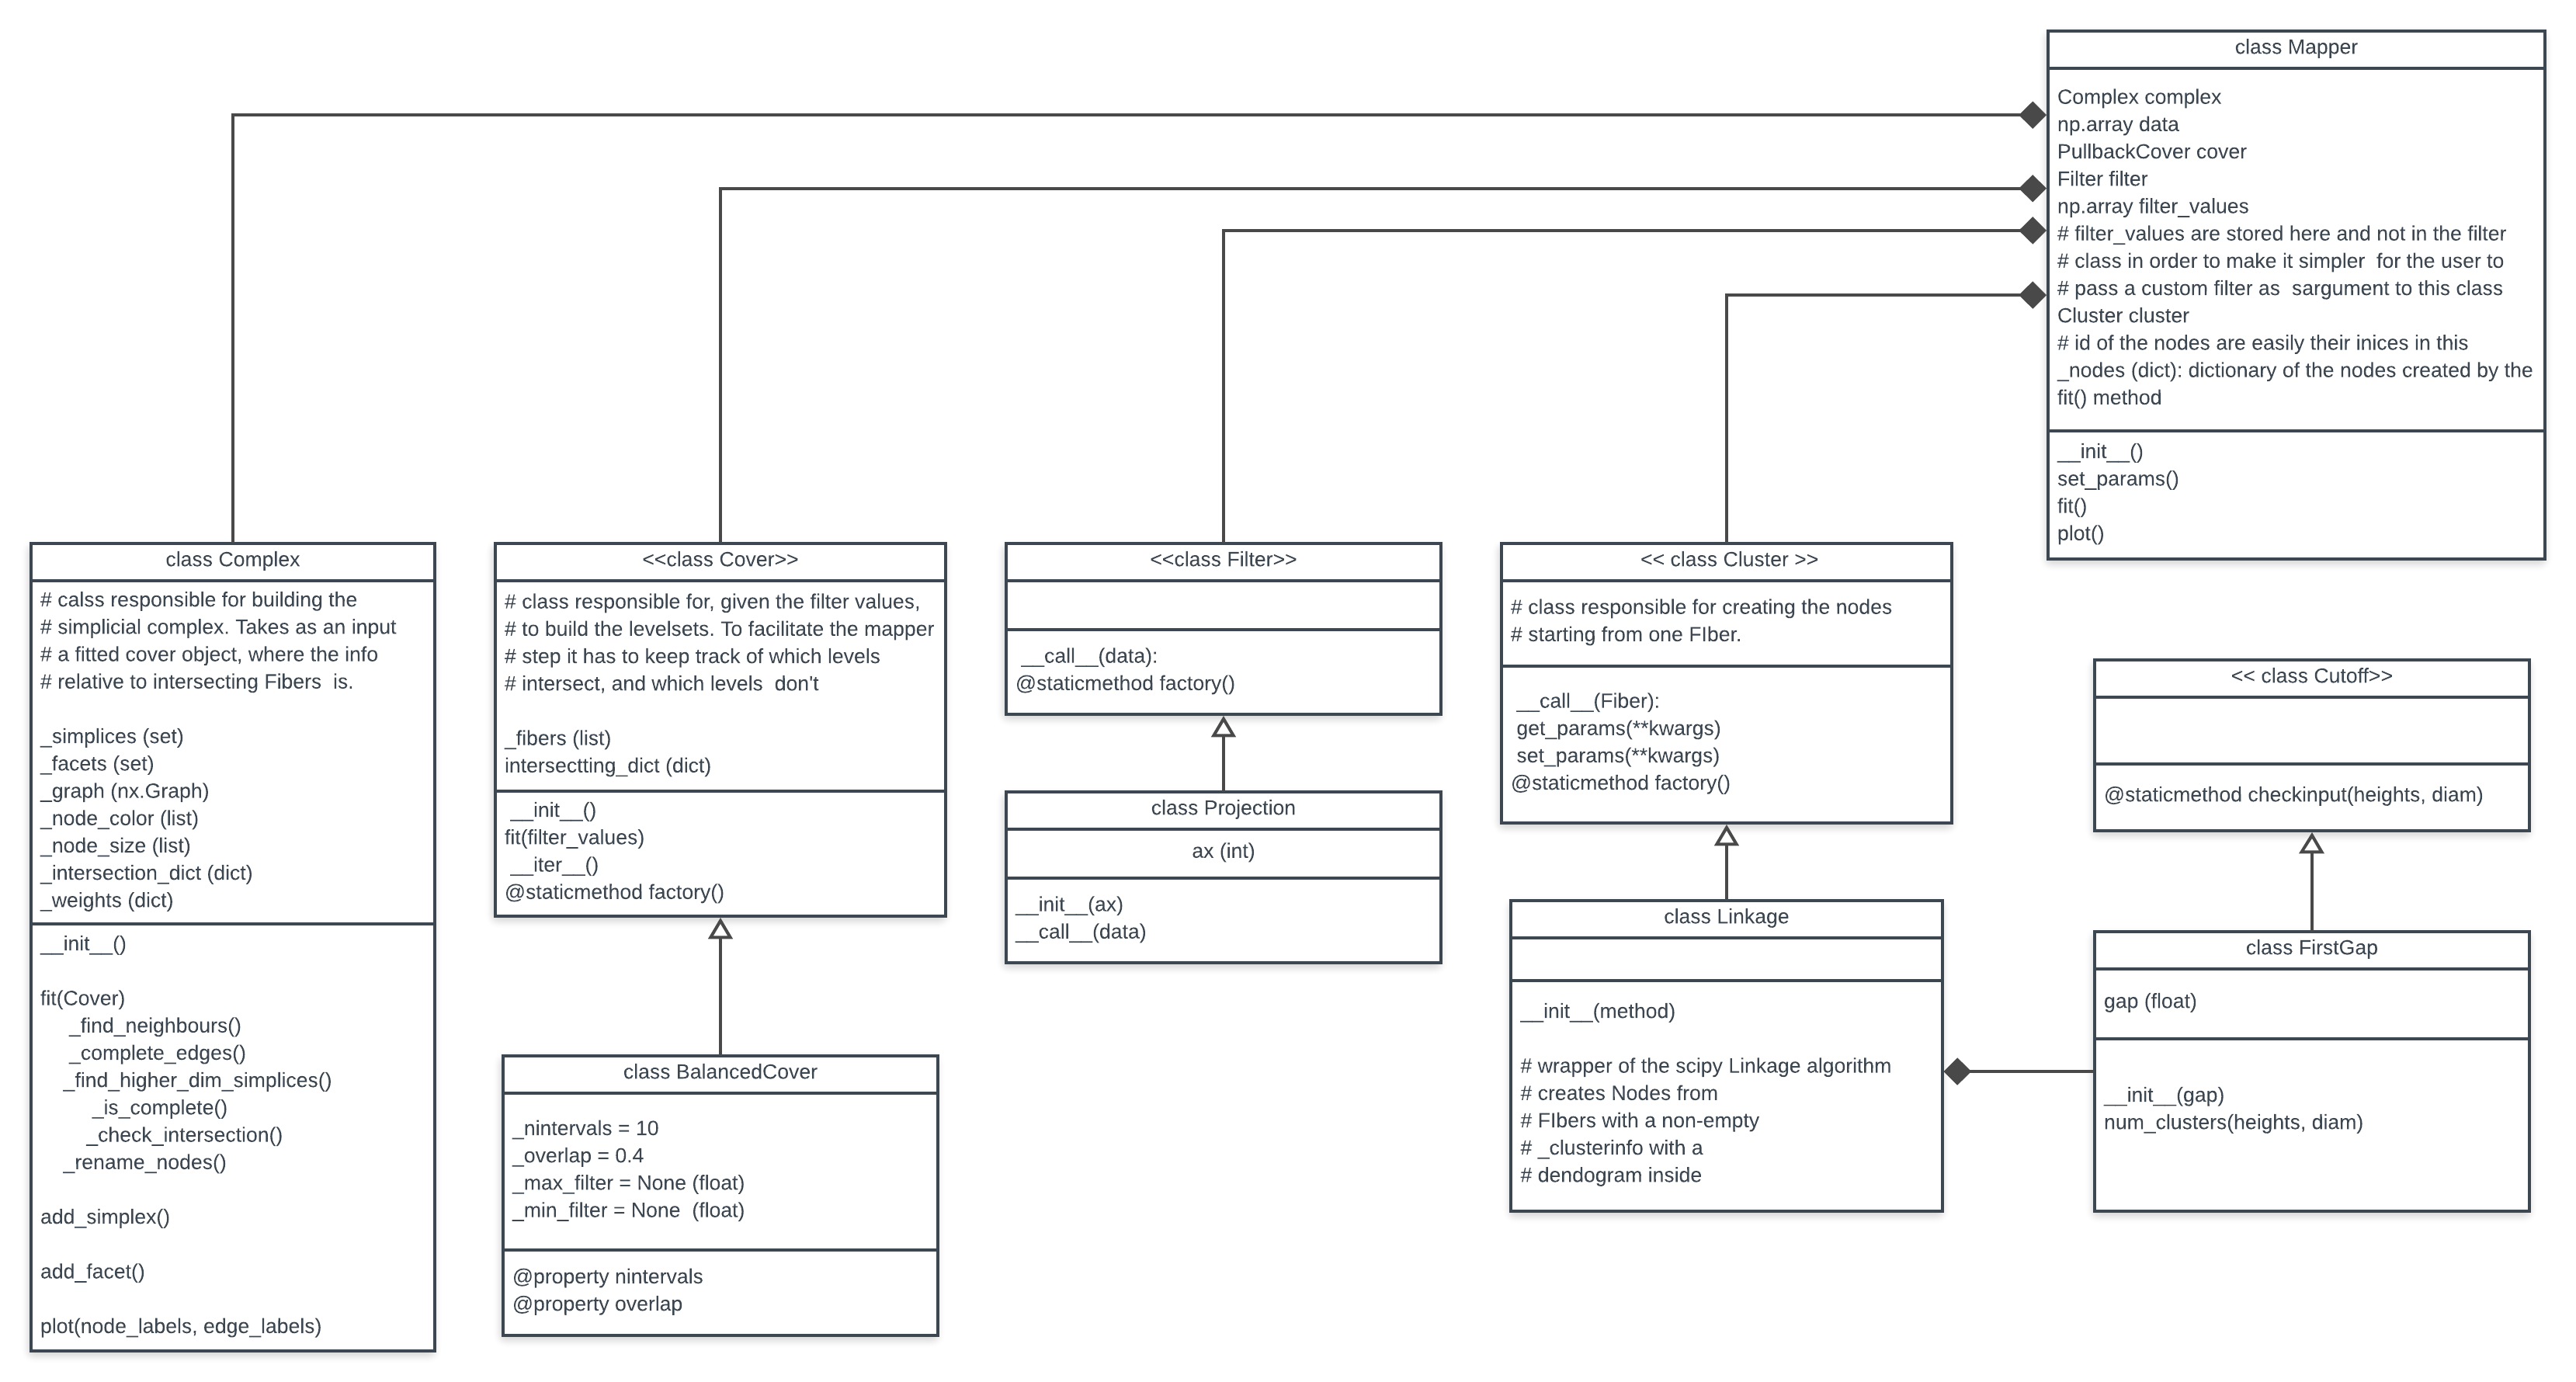
\includegraphics[width=1\textwidth]{Figs/SimplifiedArchitecture.png}
	\label{fig:basearchitecture}
\end{figure}
Three classes \textit{class Filter, class Cover, class Cluster} defining the API of the backend of the package are defined, one for each of the first three steps of the Mapper pipeline. Every class implementing an algorithm for a pipeline step has to derive from one of these classes,  in order to be compatible with the package. \textit{class Complex} is responsible for the fourth and last step of the Mapper pipeline. The classes exposed to the user would be only \textit{class Mapper, class Projection, class BalancedCover, class Linkage}. All the other classes, explained in detail later on, will be part of the backend of the package, and thus should not be used in any client code.

\subsection{Description of the classes}
In figure \ref{fig:fullmapperarchitecture} we present the UML graph of the final version of the package.
\begin{figure}[h]
	\caption{Full Mapper Architecture}
	\centering
	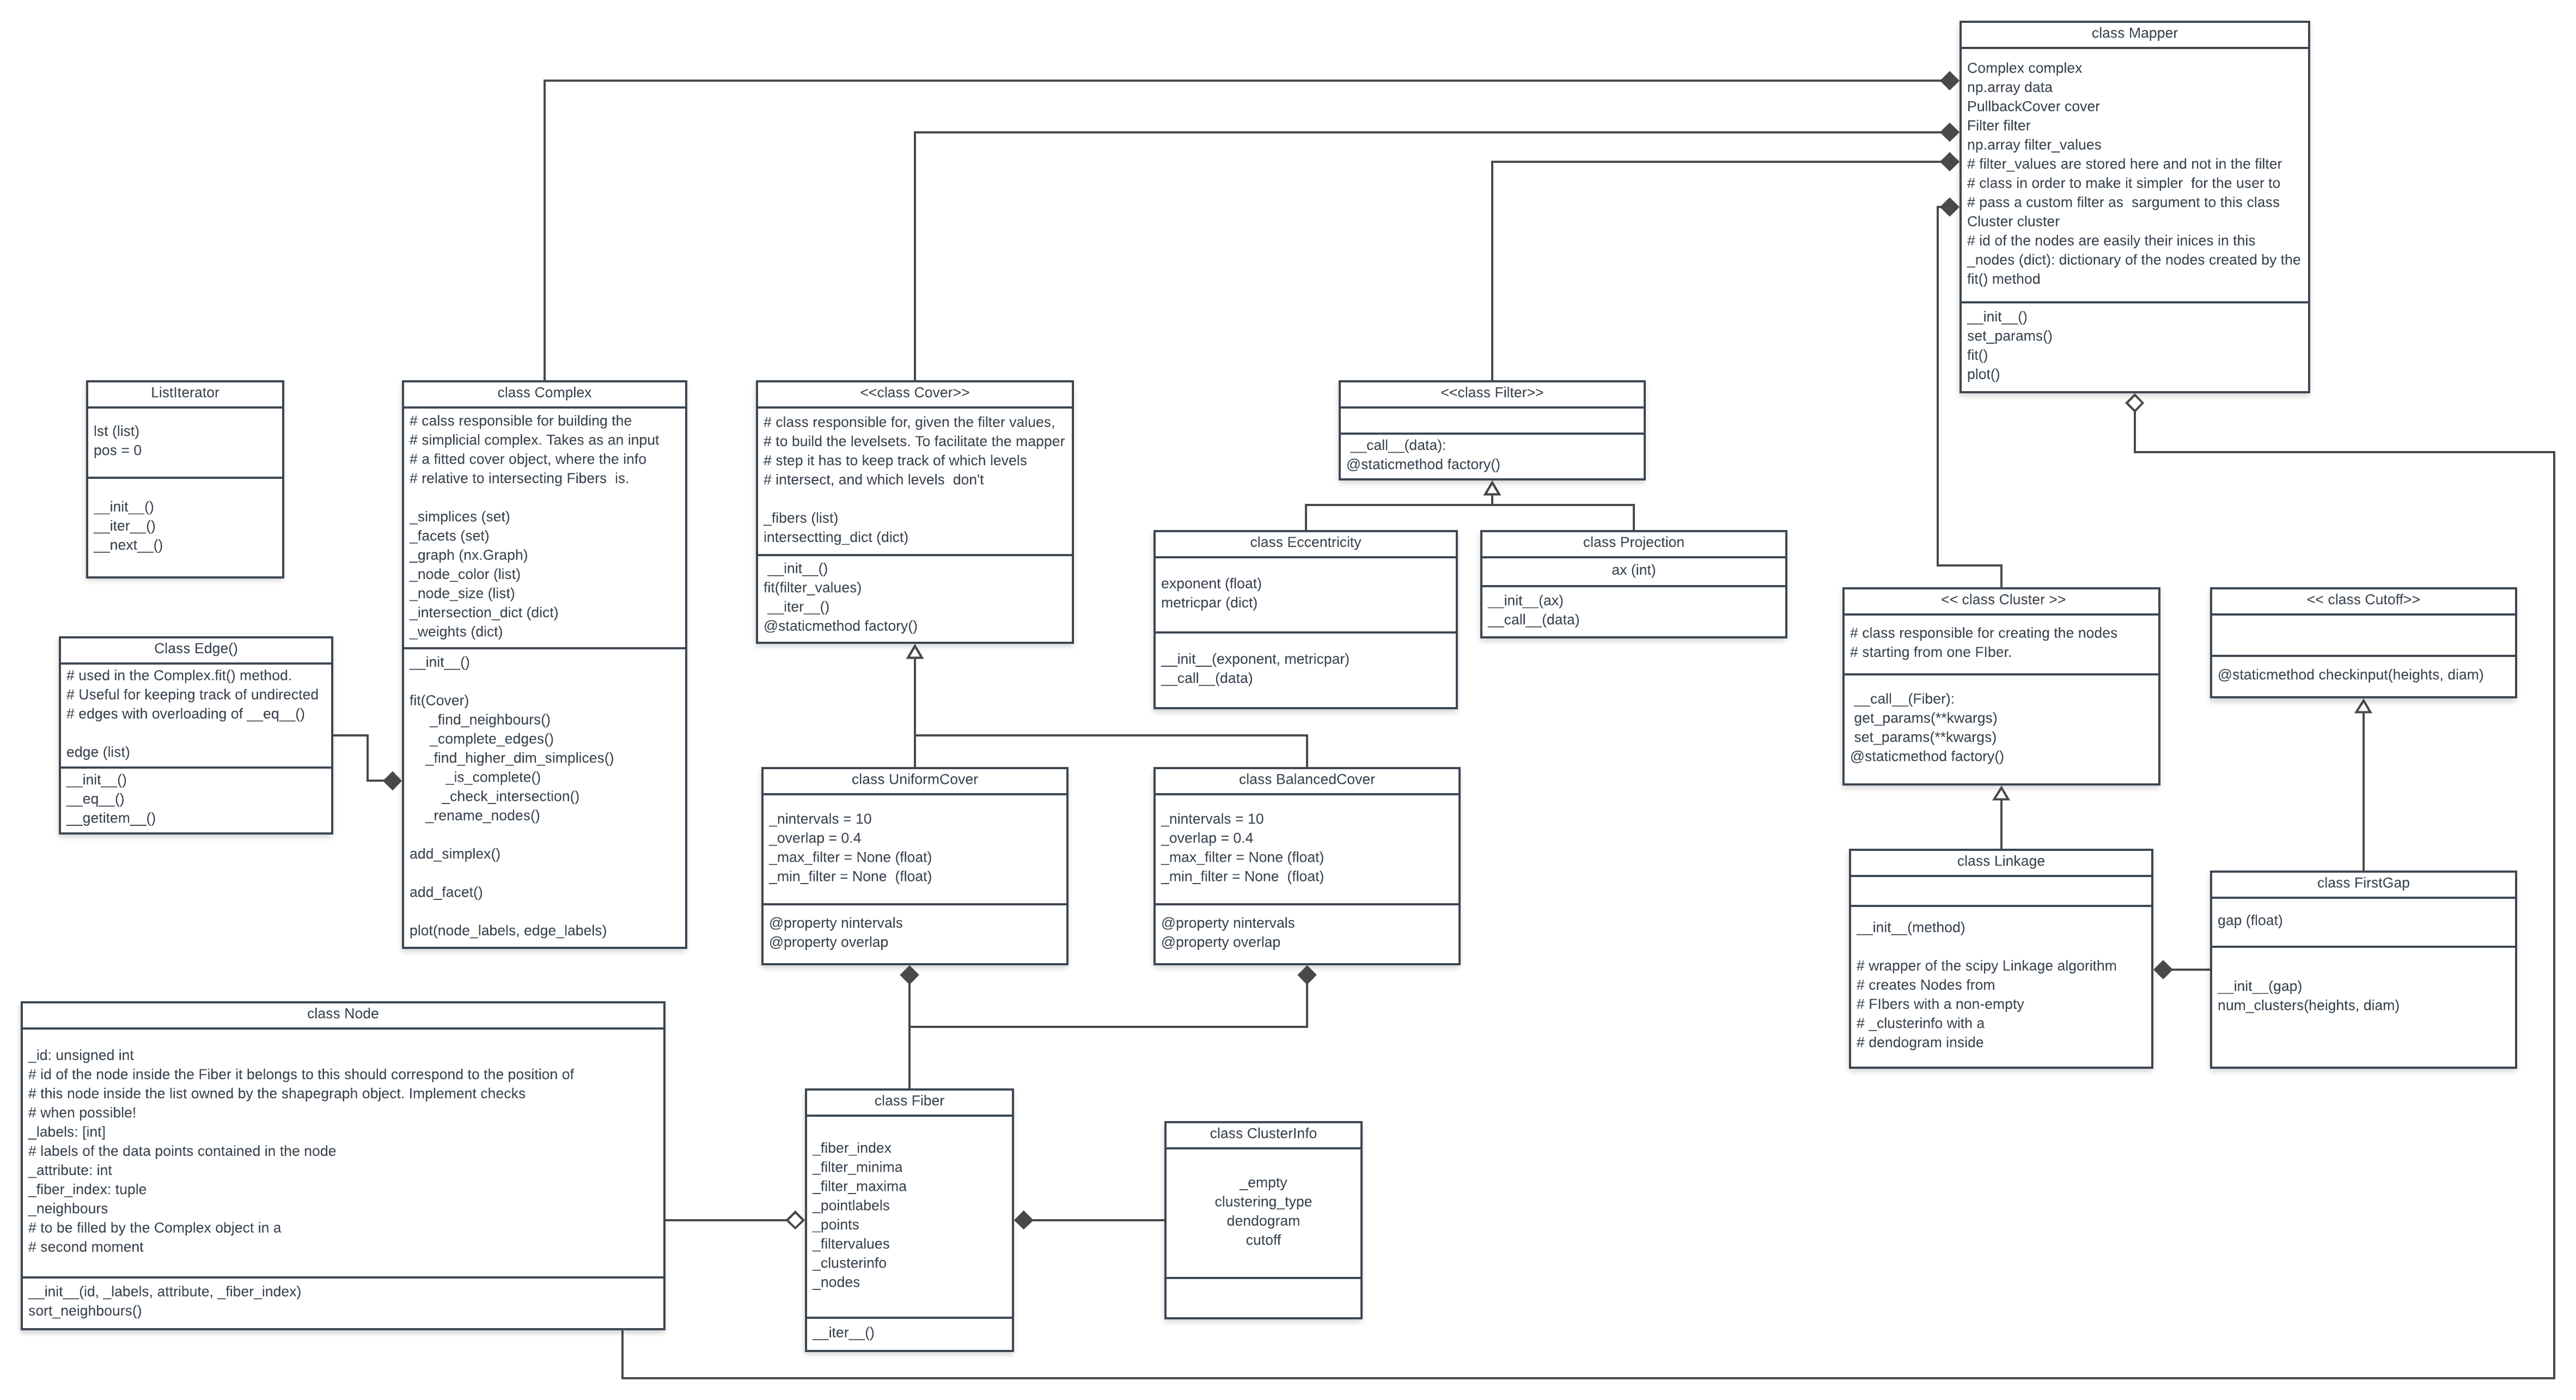
\includegraphics[width=1\textwidth]{Figs/fullMapperArchitecture.png}
	\label{fig:fullmapperarchitecture}
\end{figure} 
In this section we present the classes in a top-to-bottom order in order to first present the classes implementing the most high level algorithms, and only at the end present the classes implementing the low level details.

\subsubsection{\textit{class Mapper}}
\begin{lstlisting}[language=Python, caption=Example for the Mapper class]
import lmapper as lm
from lmapper.filter import Projection
from lmapper.cover import UniformCover
from lmapper.cluster import Linkage
from lmapper.cutoff import FirstGap
from lmapper.datasets import circles

filter = Projection(ax=0)
cover = UniformCover(nintervals=15,
                   overlap=0.4)
cluster = Linkage(method='single',
                 cutoff=FirstGap(0.05)
mapper = lm.Mapper(data=circles,
                   filter=filter,
                   cover=cover,
                   cluster=cluster)
mapper.fit()
mapper.plot()
\end{lstlisting}

\begin{lstlisting}[language=Python, caption=Example 2 for the Mapper class. The Mapper object can be initialized just with the data matrix.]
import lmapper as lm
from lm.datasets import circles

mapper = lm.Mapper(data=circles)
mapper.fit()
mapper.plot()
\end{lstlisting}

\begin{lstlisting}[language=Python, caption=Example 3 for the Mapper class. The arguments of the init function can be strings.]
import lmapper as lm
from lm.datasets import circles

mapper = lm.Mapper(data=circles,
										filter='Projection',
										cover='UniformCover',
										cluster='Linkage')
mapper.fit()
mapper.plot()
\end{lstlisting}

\begin{lstlisting}[language=Python, caption=Example 4 for the Mapper class. The filter given to the init function of the Mapper object can be a Python function.]
import lmapper as lm
from lmapper.cover import UniformCover
from lmapper.cluster import Linkage
from lmapper.cutoff import FirstGap
from lmapper.datasets import circles

def ProjectionOnFirstCoordinate(x):
	return x[:, 0]
	
cover = UniformCover(nintervals=15,
										 overlap=0.4)
cluster = Linkage(method='single',
								 cutoff=FirstGap(0.05)

mapper = lm.Mapper(data=circles,
										filter=ProjectionOnFirstCoordinate)
mapper.fit()
mapper.plot()
\end{lstlisting}


As shown in the example he Mapper init method requires four arguments: the data matrix as a two-dimensional numpy array, where the $n-th$ row represents the coordinates of the $n-th$ data point; the filter object, the cover object, and the cluster object. //
We present now the main original features of this implementation of the Mapper algorithm, that haven't been implemented neither in Kepler Mapper neither in Python Mapper.

\paragraph{Optimized calls to fit()}
The main feature of this implementation is that it is optimized for minimizing the computational time required for multiple calls to the fit() method. Since there's no way of algorithmically test the goodness of a Mapper parameters set, the only way to find a good combination of parameters is to manually explore the parameter space and observing the corresponding output graph. This is illustrated in the following example.

\begin{lstlisting}[style=mystyle, deletekeywords={filter}]
import lmapper as lm
from lmapper.filter import Projection
from lmapper.cover import UniformCover
from lmapper.cluster import Linkage
from lmapper.cutoff import FirstGap
from lmapper.datasets import circles

filter = Projection(ax=0)
cover = UniformCover(nintervals=15,
								   overlap=0.4)
cluster = Linkage(method='single',
						   cutoff=FirstGap(0.05)

mapper = lm.Mapper(data=circles,
								 filter=filter,
								 cover=cover,
								 custer=cluster)
mapper.fit()
mapper.plot()

# we want to see what happens if we change the clustering step
# from a Single Linkage to an Average Linkage,
# mantaining all the rest of the Mapper parameters equal. 
# For this purpose we use the set_params() method

mapper.set_params(cluster= Linkage(method='average', cutoff=FirstGap(0.05))

# After having changed the parameters, we need to fit the Mapper object
mapper.fit()

# Now we can plot the new mapper graph to compare it with the previous one
mapper.plot()
\end{lstlisting}

Since in practice it is normal to alternate many calls to fit() and set\_params() to find a good parameter set, the fit() method has been implemented in order to avoid to alway recompute everything from scratch. The Mapper algorithm has indeed a clear pipeline presented in section 2.1. If as in the example above we change only the parameters of the clustering step, it is useless to recompute the filter values and the cover, already calculated before. For this reason, the Mapper class keeps track internally of its state, what has changed compared to the previous state, and the new call to the fit() method performs only the computations needed. In the example, only the clustering step will we done before computing the output graph.
\subsubsection{\textit{class filter.Filter}} \label{subsubsection:class filter.Filter}
Python do not provide the opportunity of defining abstract classes. However, given the non trivial complexity of the package, we chose to the define anyway a base class for each step of of the Mapper pipeline to provide a clear way of understanding the interface of the backend API. \textit{Each one of these four classes} \lstinline{class filter.Filter, class cover.Cover, class cluster.Cluster, class cutoff.Cutoff} \textit{was written in order that every time a new filter, cover, cluster, cutoff has to be implemented, it will be implemented as a class derived from one of these corresponding base classes}. For example, a projection filter has to be implemented as child class of the corresponding Filter class: \lstinline|class Projection(Filter)|. For example, the programmer that will be expanding the package by adding a new filter, will have to read the code of the Filter class to see which methods have to be overridden, and which methods are already provided in the base class. In this way these four base classes act as a guideline for the programmer to make sure that every newly added class will respect the backend API of the package.\\The class Filter simply declares the \lstinline{__call__()} operator raising a \lstinline{NotImplementedError} exception, indicating to the programmer that any new filter has to override such a method. Since Python is not type-checked (although the package \textbf{typing} could be used from Python 3.5) it was chosen to put clear indications of the expected parameter and the return value type In the docstring of the \lstinline{filter.Filter.__call__()} method. The same procedure has been used for all the methods of the thee other base classes \lstinline{class filter.Filter, class cover.Cover, class cluster.Cluster, class cutoff.Cutoff} raising a \lstinline{NotImplementedError} exception.\\ A static factory method necessary for the instantiation of the Filter object when the Mapper object is instantiated with only strings as arguments. Note that the code of \lstinline{filter.Filter.factory()} does not have to be updated every time a new child class is added to the package thanks to the use of the \lstinline{globals()} method.

\subsubsection{\textit{class filter.Eccentricity(filter.Filter)}}
This implements the eccentricity filter as presented in \cite{pythonmapper}. In short, the eccentricity filter value of the $n-th$ data point is the p-norm of the $n-th$ row of the distance matrix
$$Eccentricity(x_i; p) = \left(\sum_{k=0}^{N} d(x_i, x_k)^p\right)^\frac{1}{p}$$
As explained above in section \ref{subsubsection:class filter.Filter} we can see that this class is a child of \lstinline|filter.Filter|. It implements an \lstinline|__init__()| method initializing the attributes that every cover object must have and overrides the method \lstinline|__call__()| as indicated in the docstring of the same method of the base class \lstinline|filter.Filter.__call__()|.\\
Since the computation of the eccentricity is computationally very expensive because of the calculation of the full distance matrix, the implementation of the Python functions \lstinline{eccentricity()} and \lstinline{my_distance()} were implemented in C++ and are available in the module \textbf{filterutils}. They provide an efficient parallel implementation of the most CPU-intensive part of the algorithm through the use of OpenMP.\\
When the package \textbf{lmapper} is imported, the module \textbf{filterutils} is imported. If the latter import fails, the user is notified about the failure with a printed message on the terminal and a slower, fully Python implementation of the functions \lstinline{eccentricity()} and \lstinline{my_distance()} provided in the \textbf{filter.py} module is used instead.\\
A last method, \lstinline|filter.Eccentricity.for_assignment_only()| is defined. However, this method is meant to be used from the companion package \textbf{predmap} and not to be exposed to the final user of the package. This implementation is however not clean and prone to bugs, since it makes the implementations of the two packages profoundly interdependent. This method is necessary as the \lstinline|filter.Filter.__call__()| method is meant to operate on two-dimensional \lstinline|np.ndarray| representing the whole data matrix in order to vectorize as much as possible the computations to achieve speedup. However, we'll see that in \textbf{predmap} it is necessary to compute the filter values \textit{of only one new data point belonging to the test set after having already computed the filter values of the whole original data matrix of the training set}. These two different situations of calculating filter values require two different implementations. It is not clear if the implementation needed in the second scenario was to be implemented in \textbf{predmap} or in \textbf{lmapper}. For now it has been chosen to add this method \lstinline|filter.Eccentricity.for_assignment_only()|. A more elegant solution is left as further work.

\subsubsection{\textit{class cover.Cover}}
As explained above in section \ref{subsubsection:class filter.Filter} \lstinline|class cover.Cover| is a base class to define the common interface that any new implementation of a new cover method must respect. Similar to \lstinline|filter.Filter| it implements an \lstinline|__init__()| method initializing the attributes that every cover object must have. It implements a method \lstinline{cover.Cover.find_intersecting_dict()} that outputs a dictionary that keeps track of which fibers intersect. This implementation is valid as soon as the filter values are one dimensional, and each Fiber object represents is the counter image of an interval on the real line. When the package will be expanded with multi-dimensional filters, or with more complicated ways of building a cover, this method will become obsolete and must be changed.
\subsubsection{\textit{class cover.UniformCover(OverlapCover)}}
It derives from \lstinline|class OverlapCover(Cover)|. This latter class was introduced since \lstinline|class UniformCover(OverlapCover), KeplerCover(OverlapCover), BalancedCover(OverlapCover)| share the common idea of being defined by overlapping intervals on the image of the filter $f(X)\subset\mathcal R$. We can see that  \lstinline|class cover.UniformCover(OverlapCover)| just needs to define the \lstinline{cover.UniformCover.fit()} method, in which the particular construction of this specific cover is implemented. Note that "constructing a cover" for an \lstinline{OverlapCover} means finding the variables  \lstinline|list_of_as| and  \lstinline|list_of_bs| that are respectively the list of the leftmost extremes and the rightmost extremes of the intervals $I_j=(a_j, b_j)$ forming the open cover $\mathcal I = \{I_j\}$ of $f(X)$. Once defined these intervals, all the rest of the implementation is taken care of by the method \lstinline|cover.OverlapCover.find_entries()| that finds the corresponding data points belonging to each preimage $f^{-1}(I_j)$ and instantiating an object of class \lstinline|cover.Fiber| for each preimage $f^{-1}(I_j)$. The output  of \lstinline|cover.OverlapCover.find_entries()| is a list of \lstinline|cover.Fiber| objects, and a dictionary created by the \lstinline|cover.Cover.find_intersecting_dict()| method.
\subsubsection{\textit{class cover.Fiber}}
\lstinline|class cover.Fiber| is just a data structure containing informations relative to each preimage $B_i$ of the pullback cover $\mathcal B = \{B_i\}$. It stores the indices of the data points that the corresponding preimage $B_i$ contains, their filter values, and other useful information.
\subsubsection{\textit{class complex.Node}}
Class responsible for storing the information of one node of the final complex, result of the cluster call on a Fiber. The objects of class Node are stored (owned) by objects of class Fiber and instantiated by the \_\_call\_\_()method of an object of class cluster.Cluster.
\subsubsection{\textit{class ClusterInfo}}
Data structure containing information about the parameters of the clustering algorithm used to produce the Nodes. Objects of class ClusterInfo are owned by Fiber objects. 
\subsubsection{\textit{class cluster.Cluster}}
Abstract class implementing the interface for any Cluster Object.
\subsubsection{\textit{class cluster.Linkage}}
Example of Cluster object. The \_\_cal\_\_() method takes a Fiber, accesses to its data points and cluster them. Each cluster is represented by one Node object, that is owned by the corresponding fiber in its list attribute Fiber.\_nodes.
\subsubsection{\textit{class cutoff.Cutoff}}
The Cutoff class is an abstract class providing the interface for each different cutoff object
\subsubsection{\textit{class cutoff.FirstGap}}
Example of Cutoff. This class implements the First Gap method illustrated by Carlsson et al. in \cite{PAD}. It is used by the cluster.Linkage class to determine the number of clusters to create starting from the full linkage matrix.
\subsubsection{\textit{class complex.Complex}}
Class responsible for storing all the simplices, edges, nodes of the Nerve Complex output of the Mapper algorithm. It also implements a method for drawing te 1-skeleton of the nerve complex. Starting from a Cover object the fit() method accesses all the fibers, all the corresponding nodes and looks for intersections between nodes, creating a corresponding Nerve Complex stored as a list of simplices in the \_simplices attribute. The corresponding 1-d skeleton is stored in the NetworkX.Graph attribute complex.Complex.\_graph. 

